%% Dokumentklasse KOMA-Script Report
\documentclass[paper=a4, 12pt]{scrreprt}
%% Encoding UTF8
\usepackage[utf8]{inputenc}
%% 8 Bit Aufloesung der Buchstaben
\usepackage[T1]{fontenc}
%% Seitenraender
\usepackage[scale=0.72]{geometry}
%% Spracheinstellungen
\usepackage[english, naustrian]{babel} % your native language must be the last one!!
%% erweiterte Farbenpalette
\usepackage[dvipsnames]{xcolor}
%% Abbildungen
\usepackage{graphicx}
%% Tabellen (erweitert)
\usepackage{tabularx}
%% TikZ + Circuit-TikZ (fuer Schaltungen)
\usepackage[europeanresistors, europeaninductors]{circuitikz}
%% Nuetzliche TikZ Libraries
\usetikzlibrary{arrows, automata, positioning}
%% mathematik
\usepackage{amsmath, amssymb}
%\usepackage{mathtools}	
%% pdf-einbindung
\usepackage{pdfpages}
%% scource-code einbindung
\usepackage{listings, scrhack} %scrhack vermeidet Umschaltung auf KOMA Floats..
\usepackage{courier}
%% euro-symbol
\usepackage{eurosym}
%% landcsape-seiten ermöglichen
\usepackage{lscape}

%% Diplomarbeits-Format
\usepackage{srdpdipa}

%% Abkuerzungsverzeichnis
\usepackage[]{acronym}

%% Todos
\usepackage[]{todonotes}

%% Ganttdiagramme
\usepackage{pgfgantt}

%% Subfigures
\usepackage[lofdepth]{subfig}

%% definitionen =====================================%%
\dataSchool{HTBLuVA St. Pölten}
\dataDepartment{Höhere Lehranstalt für Elektronik und Technische Informatik}
\dataSubdepartment{Ausbildungsschwerpunkte Embedded- \& Wireless Systems}
\dataSession{2015/16}

\title{Blinkschaltung}
\author{Max Musterschüler \and Otto Normalschüler}
\date{\today}
\place{St. P\"olten}
\professor{Prof. HAI \and Prof. FISCH}
%%====================================================%%

% Hyperlinks im Dokument
\usepackage[colorlinks=true,
    linkcolor=black,
    citecolor=green,
    bookmarks=true,
    urlcolor=black,
    bookmarksopen=true]{hyperref}

\begin{document}

\frontmatter

%% titelseite ==========================================%%
\maketitle
%%======================================================%%

%% komplett leere seite ================================%%
\newpage\null\thispagestyle{empty}\newpage
%%======================================================%%

%% eidesstattliche erklärung ===========================%%
\begin{affidavit}
    \unterschrift{Max Musterschüler}
    \unterschrift{Otto Normalschüler}
\end{affidavit}
%%======================================================%%

%% dokumentation (deutsch/englisch) ====================%%
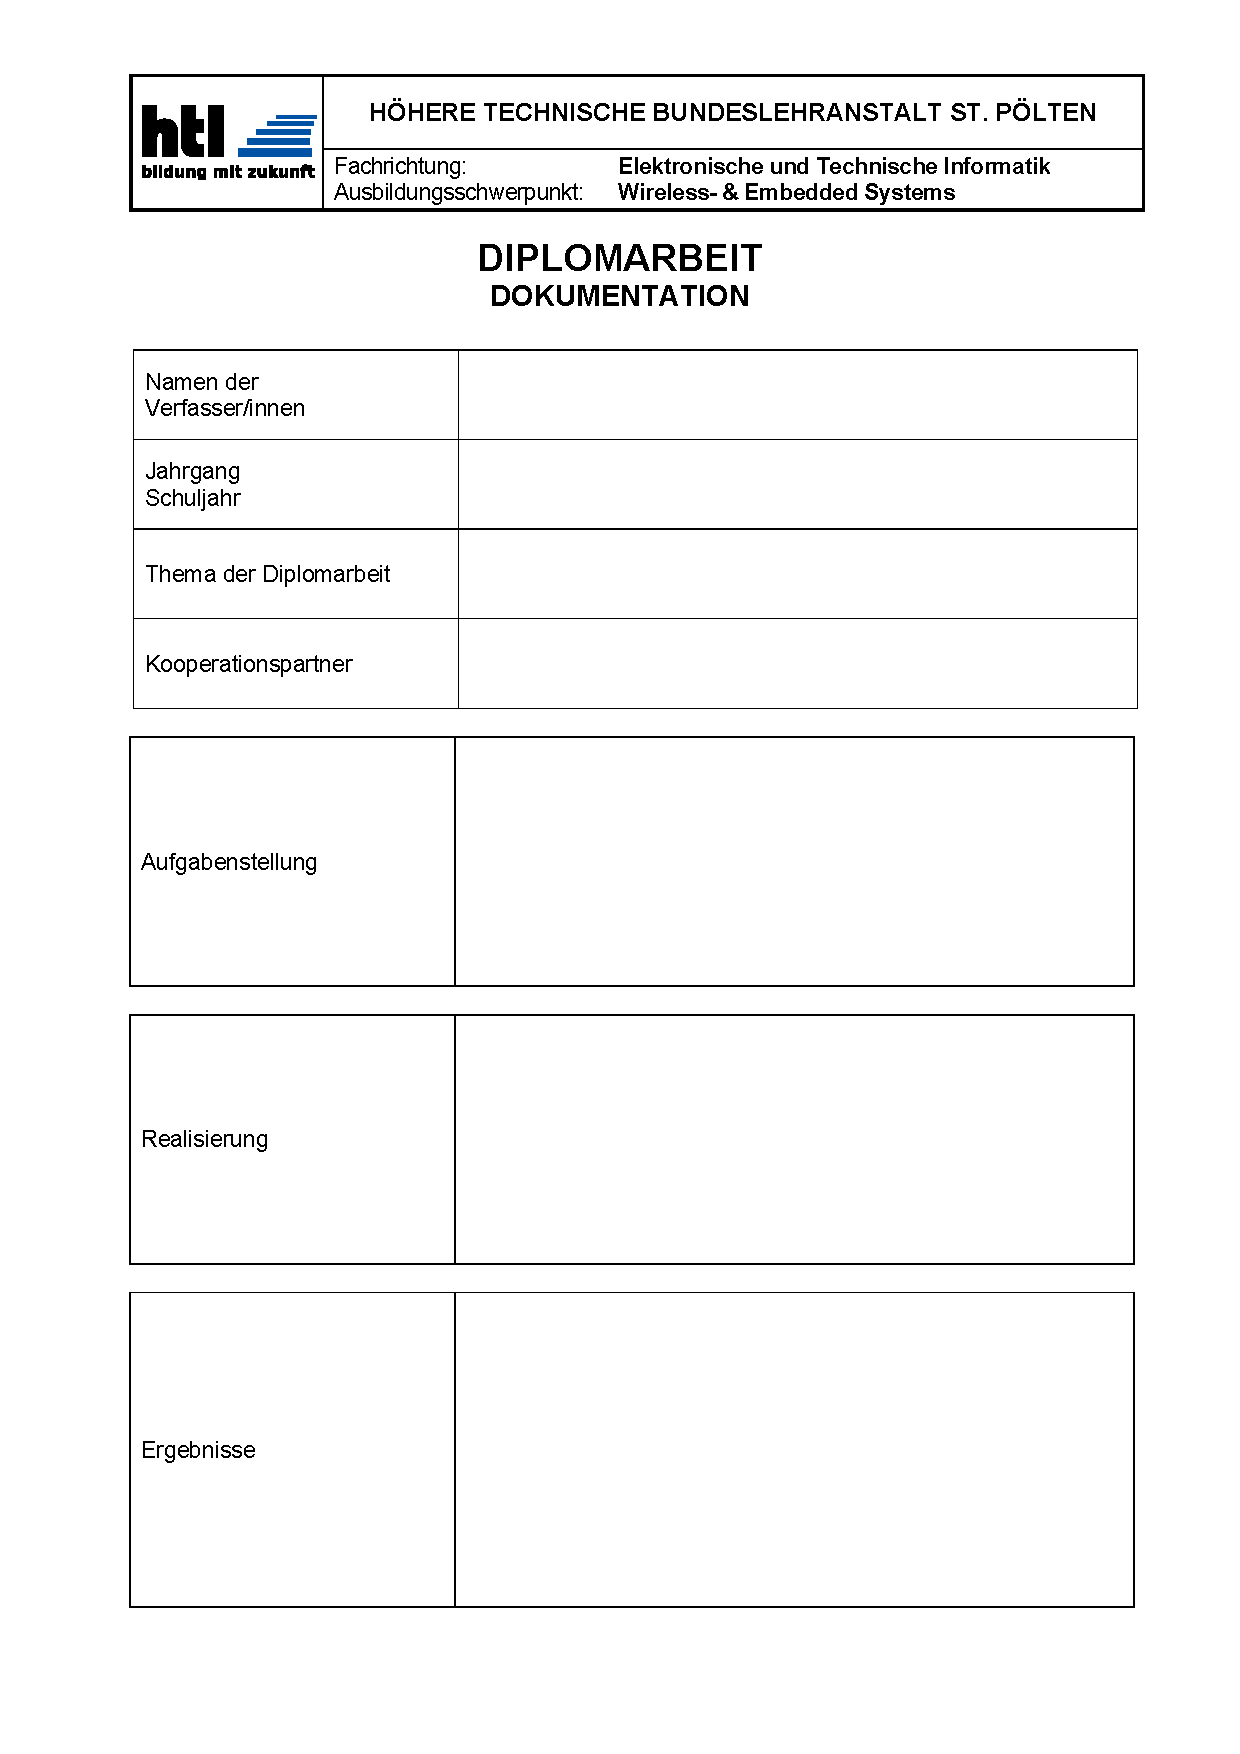
\includepdf[pages=-]{form/dokumentation-de.pdf}
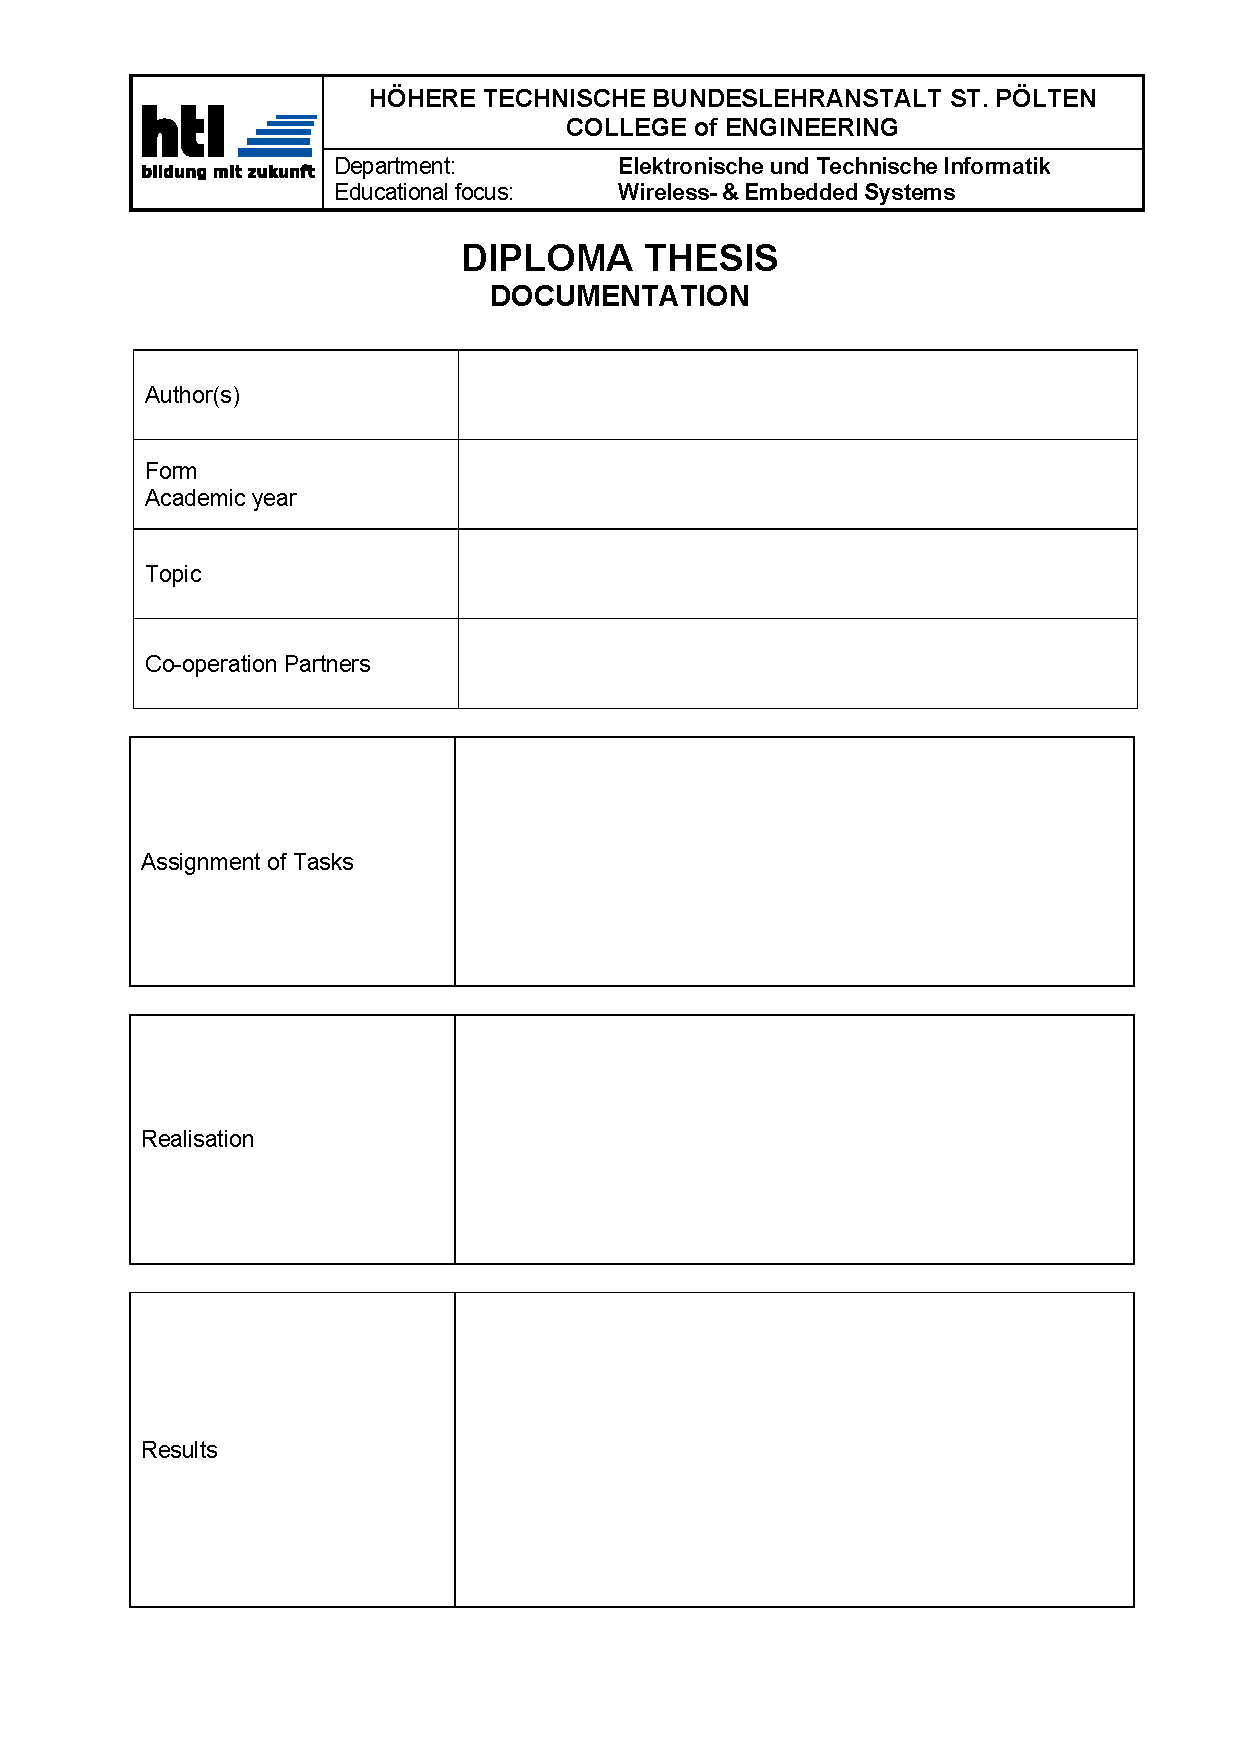
\includepdf[pages=-]{form/dokumentation-en.pdf}
%%======================================================%%

%% inhaltsverzeichnis ==================================%%
\tableofcontents
%%======================================================%%

%% HAUPTTEIL ===========================================%%
\responsible{Max Musterschüler, Otto Normalschüler}
\mainmatter

\chapter{chapter}
\section{section}
\subsection{subsection}
\subsubsection{subsubsection}
\paragraph{paragraph}
\subparagraph{subparagraph}

\chapter{Einleitung}
    Hier ist die Einleitung

\chapter{Individuelle Zielsetzung}
    \section{HF-Teil}
        Dieser Teil wurde von Max Musterschüler entwickelt. das ist ein test von git
    
    \section{Filter}
        Dieser Teil wurde von Otto Normalschüler entwickelt.

\chapter{Grundlagen und Methoden}

\chapter{Ergebnisse}


%% ANHANG ==============================================%%
\appendix

%% abkürzungsverzeichnis ===============================%%
%% start of file abkuerzungen.tex

% Abkuerzungsverzeichnis
\addchap{
	\iflanguage{english}{Acronyms}{Abkürzungsverzeichnis}}
\begin{acronym}[ACRONYM]
\acro{tikz}[TikZ]{\TikZ{} ist kein Zeichenprogramm}
\acro{spi}[SPI]{Serial Peripheral Interface}
\end{acronym}\newpage

%% end of file abkuerzungen.tex
%%======================================================%%

%% abbildungsverzeichnis ===============================%%
\setcounter{lofdepth}{2}
\dipalistoffigures
%%======================================================%%

%% tabellenverzeichnis =================================%%
\setcounter{lotdepth}{2}
\dipalistoftables
%%======================================================%%

%% danksagungen=========================================%%
\begin{acknowledgements}
    Wir bedanken uns bei
    \subparagraph{Prof. Dipl.-Ing. ABCD} für ...
    \subparagraph{FL Ing. DEFG} für ...
\end{acknowledgements}

%%======================================================%%

%% literaturverzeichnis ================================%%
\newpage
\begin{literature}
% The TeXbook by D. E. Knuth
\bibitem[1]{TeXbooooook}{\textbf{Donald~E.~Knuth:} \emph{The \TeX{}book}. 1986, {\scshape Addison--Wesley} Verlag,\\ ISBN-13: 978-0-201-13447-6}

\end{literature}
 
%%======================================================%%

%% betreuungsprotokolle ================================%%
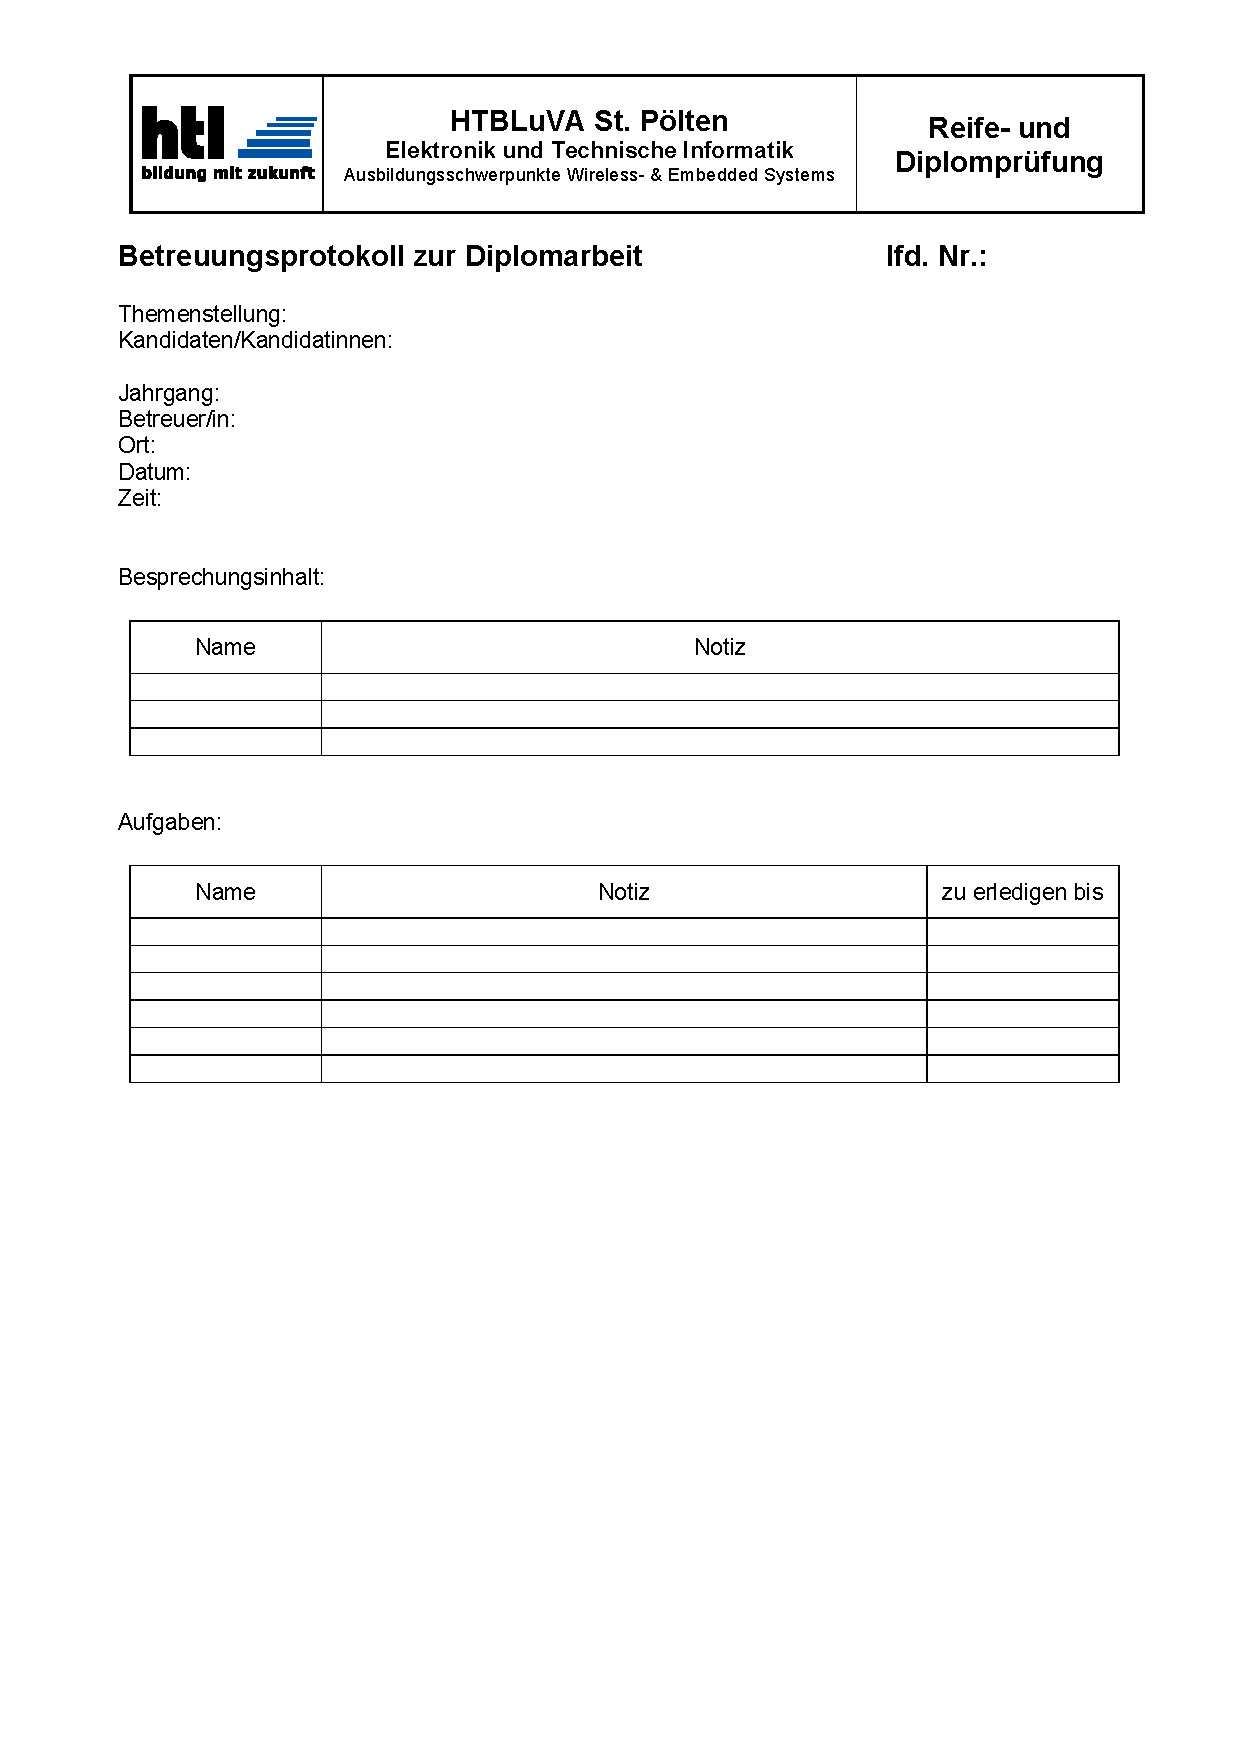
\includepdf[pages=-]{form/betreuungsprotokoll_1.pdf}
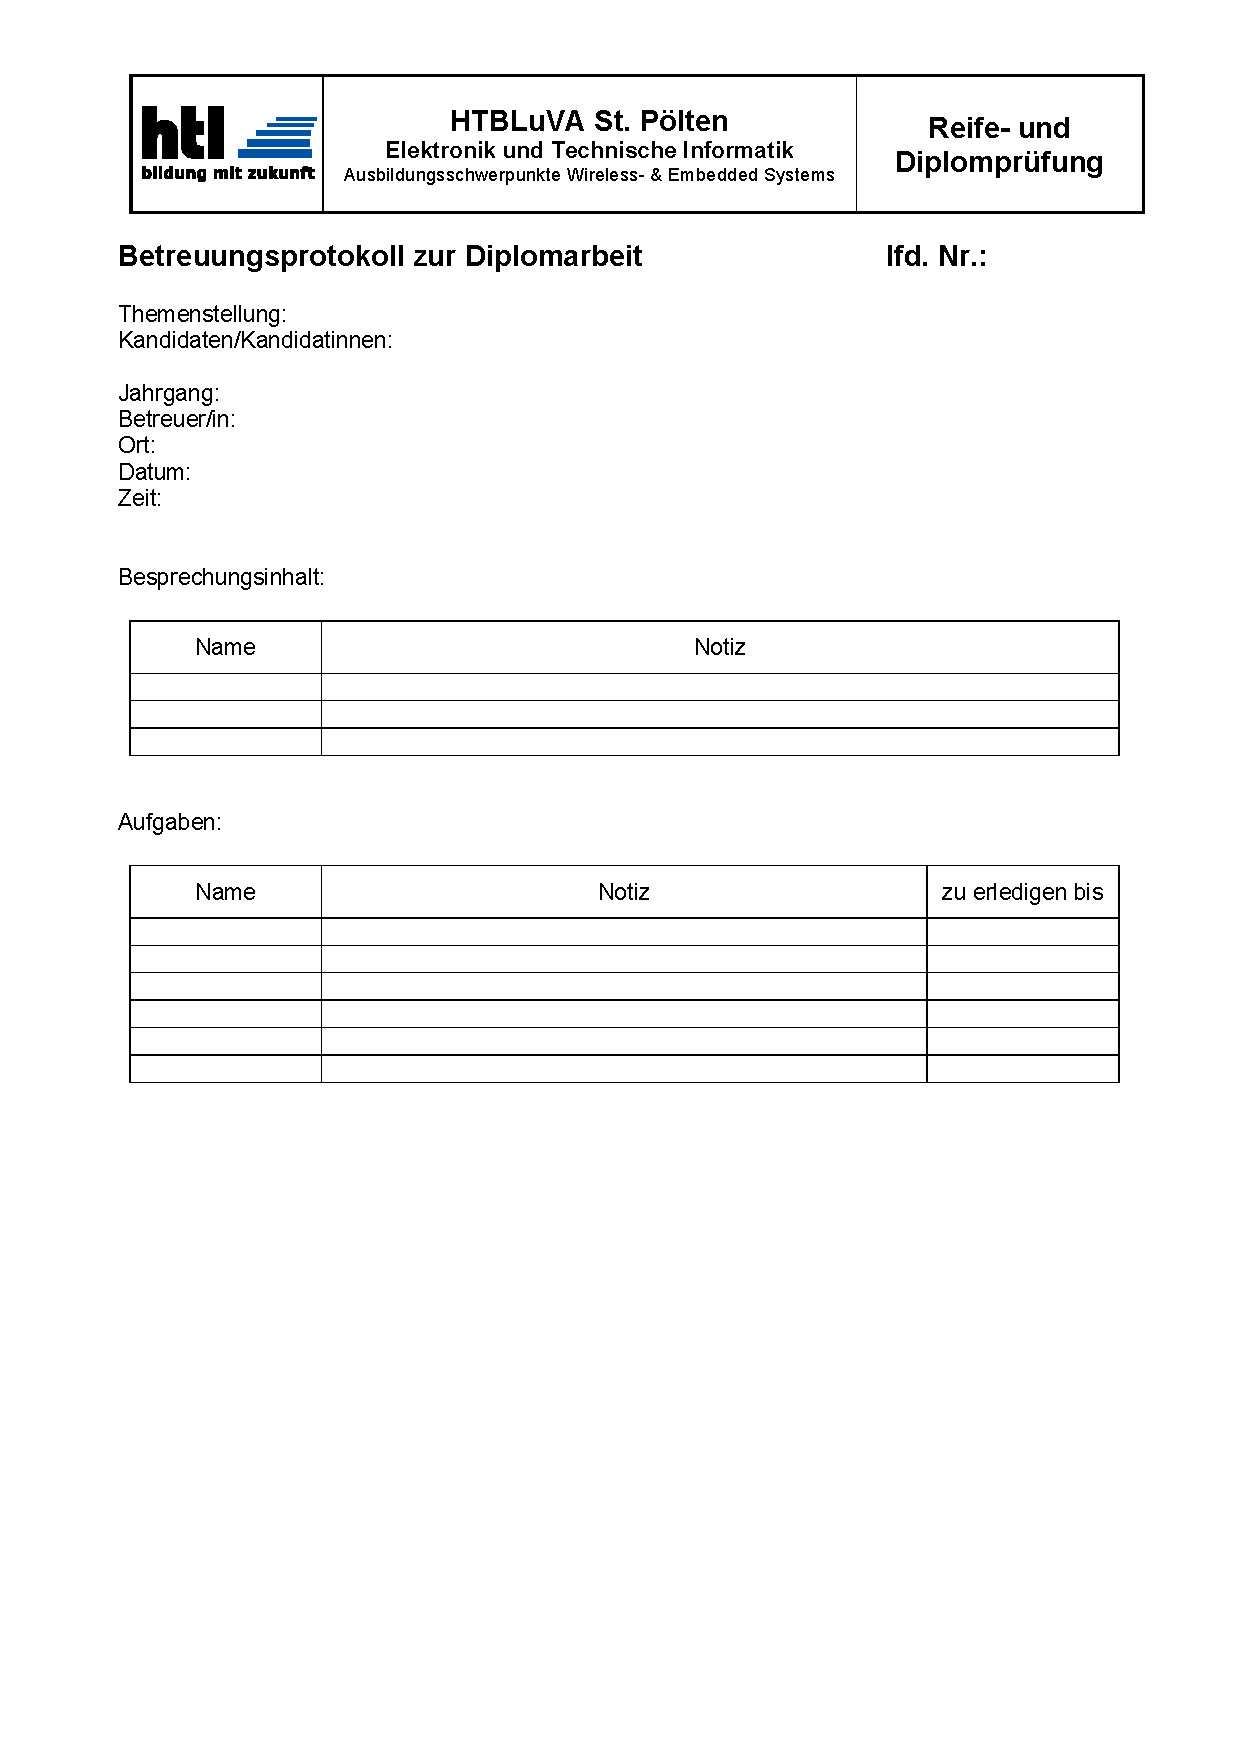
\includepdf[pages=-]{form/betreuungsprotokoll_2.pdf}
%% =====================================================%%

\end{document}
